\documentclass[11pt, a4paper]{article}
\usepackage[utf8]{inputenc}
\usepackage[left=3cm, right=3cm, top=2.5cm, bottom=3.0cm]{geometry}
\usepackage{amsmath, amssymb, amsthm}
\usepackage[english]{babel}
\usepackage{graphicx}
\usepackage[font={small,it}]{caption}
\graphicspath{ {figures/} }
\usepackage{url}
\usepackage{multirow}
\usepackage{titling}
\usepackage{subcaption}
\usepackage{wrapfig}
\usepackage[toc,page]{appendix}
\usepackage{float}
\usepackage[bottom]{footmisc}
\usepackage{titling}
\usepackage[numbered,autolinebreaks,useliterate]{mcode}

%\setlength{\droptitle}{-10em}  

\title{ \huge Artificial Neural Networks \\ 
  { \large Project 1: Regression and Classification with MLPs }}
\author{
        Lood, Cédric \\
        \small Master of Bioinformatics
}

\begin{document}
\maketitle
%\tableofcontents

\section{Context}

The analysis presented in this report was done for the class of
Artificial Neural Networks at KU Leuven (Spring 2016). It consists in
practical implementations of Multi-layer perceptrons (MLP) to solve
regression and classification problems in a supervised setting, with a
brief foray into unsupervised learning for dimensionality
reduction. The implementation was done in the MatLab environment
(2015a) using the neural networks toolbox. The scripts for each of the
sections can be found in the annex to this report.

\section{Regression}

\begin{wrapfigure}{r}{0.5\textwidth}
  \vspace{-20pt}
  \centering
  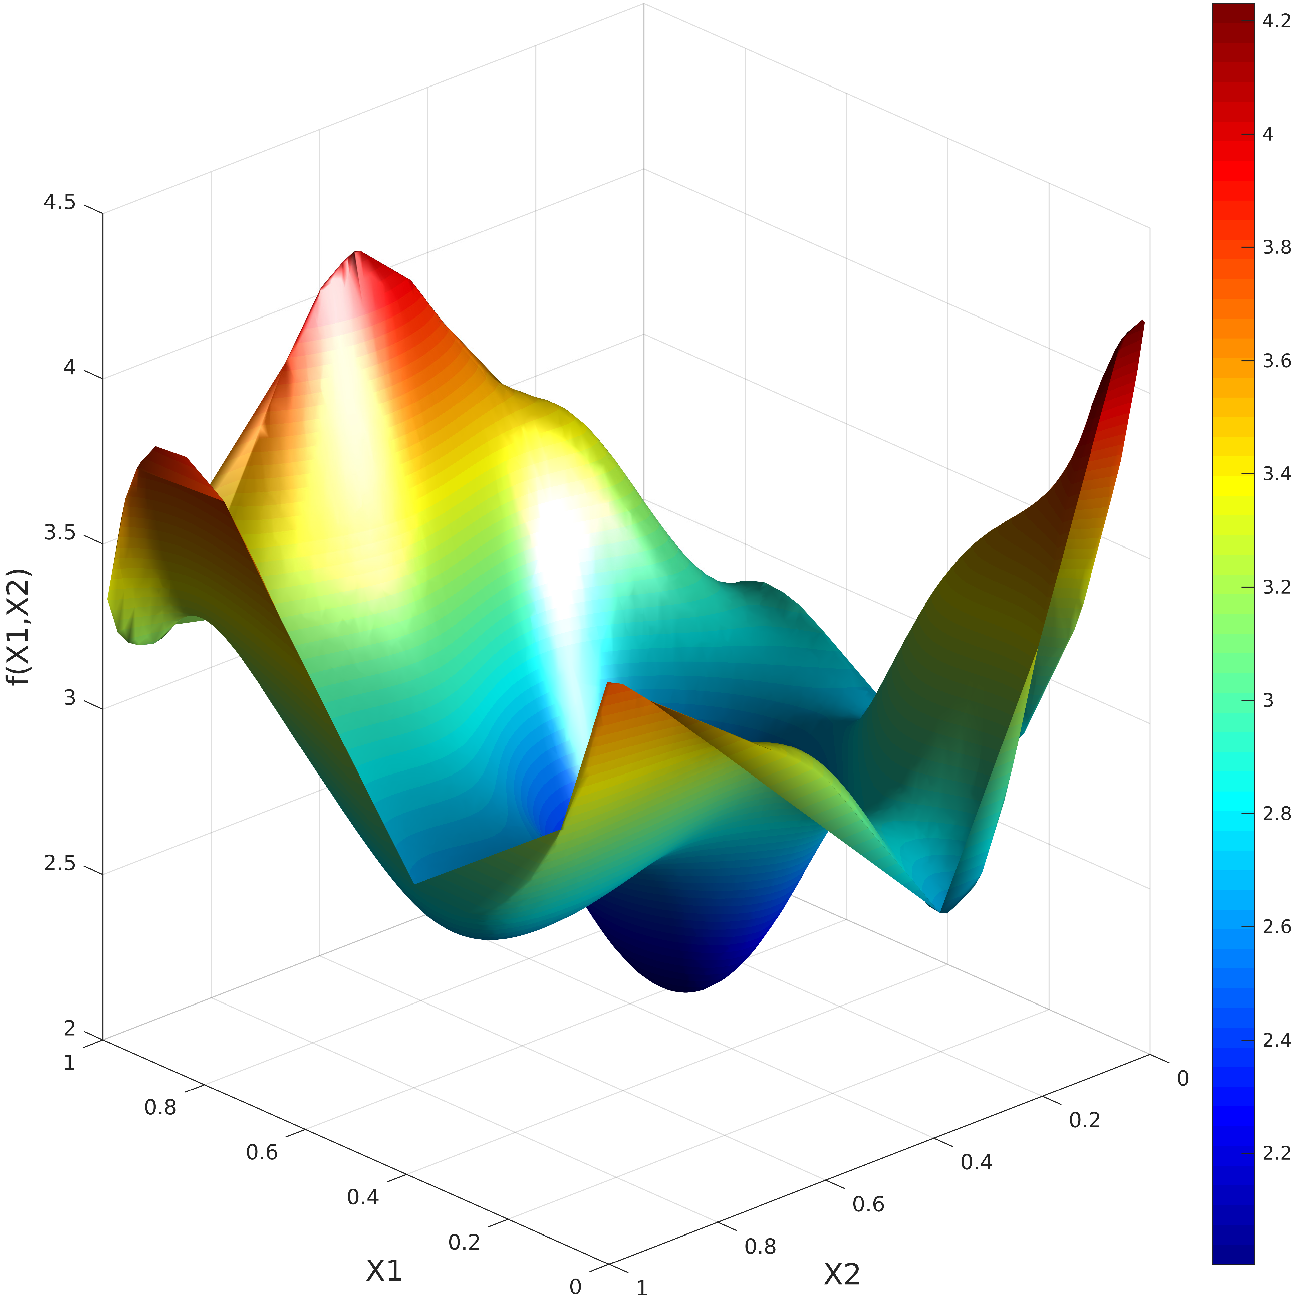
\includegraphics[scale=.35]{regression_dataset.pdf}
  \caption{Visualization of the full dataset}
  \label{fig:regression_dataset}
\end{wrapfigure}

% \begin{wrapfigure}{r}{0.5\textwidth}
%   \vspace{-20pt}
%   \begin{center}
%     \includegraphics[width=0.48\textwidth]{gull}
%   \end{center}
%   \vspace{-20pt}
%   \caption{A gull}
%   \vspace{-10pt}
% \end{wrapfigure}

The problem we need to solve here is to estimate a (unknown)
non-linear function from a given dataset of 13600 datapoints uniformly
sampled. Importantly to note, the sampled data is noiseless. The
dependent variable was generated using the student number (r0575791)
and the two dependent variables $X_1, X_2 \in [0, 1]$ (figure
\ref{fig:regression_dataset} for a rendering of the dataset
generated).

For the creation of the training, validation, and test set, I first
randomized the dataset and then proceeded to use the built-in matlab
function \emph{dividerand} which creates 3 lists of non-repeating
indices of size 1000 that can then be used to subset the original
dataset into the 3 subsets. The visualization of the sets on figure
\ref{fig:regression_traindataset} reassures that the sampling was done
correctly.

Although it is possible to use more than one layer for MLPs, I limited
myself here at 1 hidden layer, comforted by the fact that they consist
of universal approximator given that I used a non-linear transfer
function. I also obtained good results previously (see homework 1) for
function approximation using a single hidden layer. The choices I was
faced with to optimize the architecture are the number of hidden
units, the transfer function, and the choice of the training
algorithm. For the rest, the network has 2 input neurons connected to
the hidden neurons, whose outputs are linearly combined by a single
output neuron.

\begin{figure}[H]
%\vspace{-20pt}
  \centering
  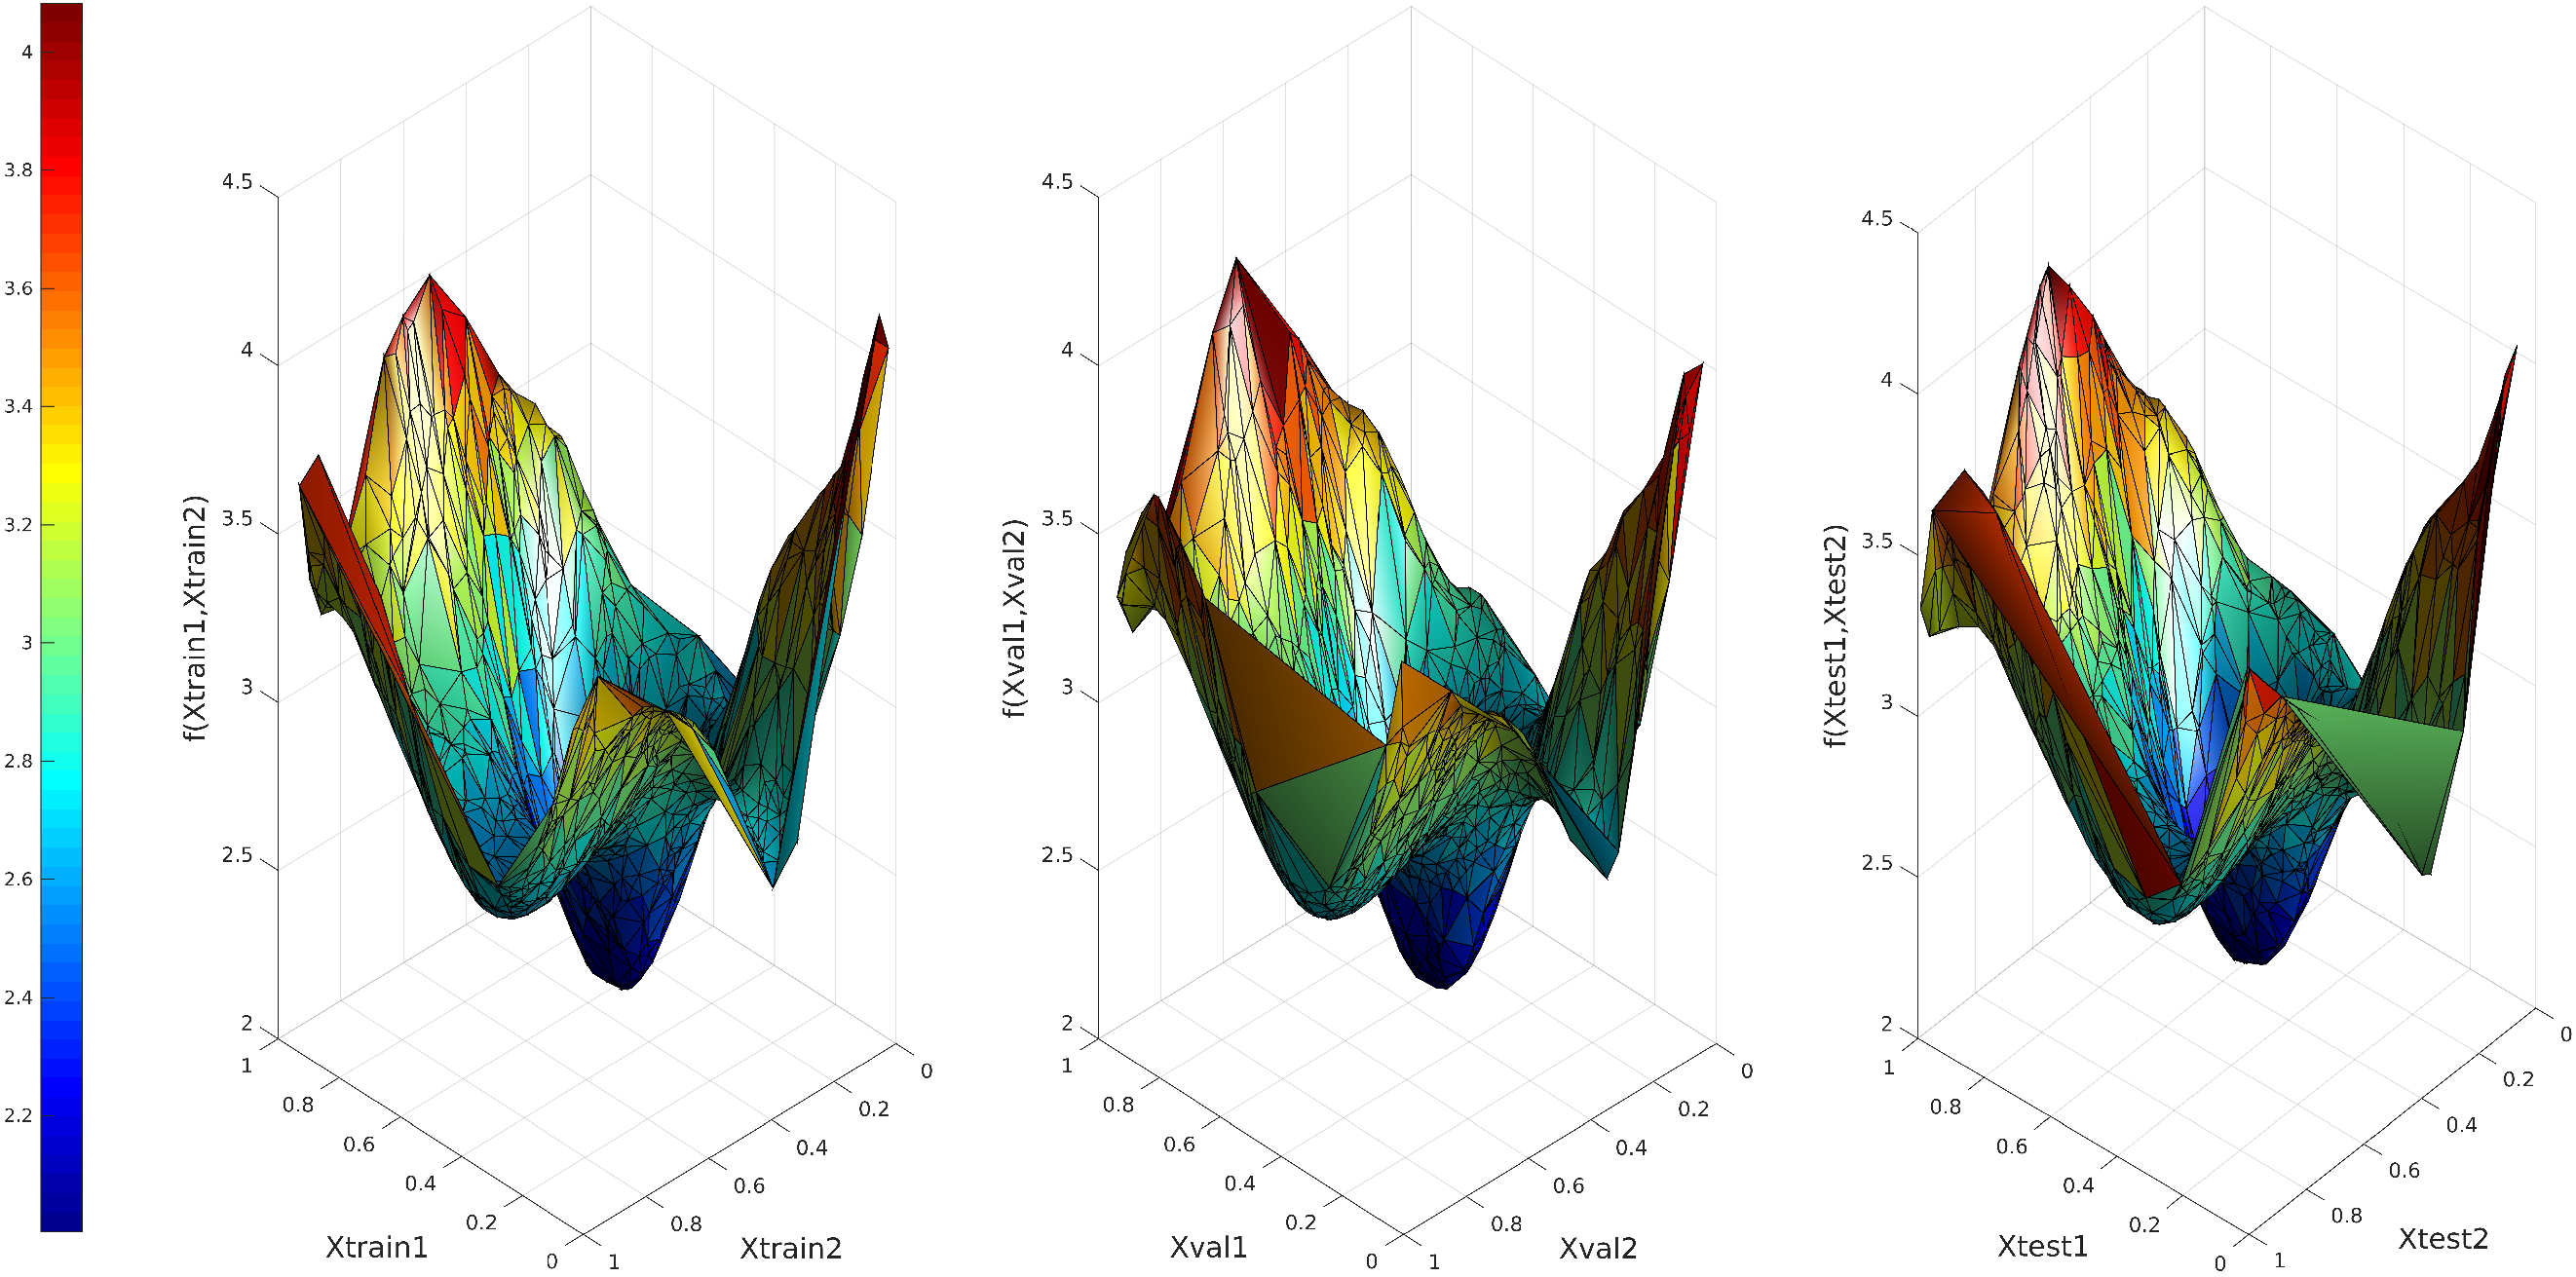
\includegraphics[scale=.30]{regression_trainingsets.pdf}
  \caption{From left to right: training, validation, and test datasets
    (1000 points each)}
  \label{fig:regression_traindataset}
\end{figure}

For the training algorithm, I based my choice on consideration such as
the size of the dataset. Since I worked on an interactive computing
node of the VSC \footnote{Vlaams Super Computer}, I did not have to
worry to much about the memory requirements (even though a 1000x1000
Hessian matrix can also be handled by a laptop computer without any
troubles), and did not investigate conjugate gradient
methods. Instead, I chose to focus on the Levenberg-Marquardt method,
which is known for its fast convergence.

On the figure \ref{fig:test_mse_error}, I report the finding in terms
of validation MSE (no usage of the training set at this stage). I
performed a systematic search for the correct amount of hidden neurons
using \emph{transig} and \emph{logsig}. On the same figure, the Test
MSE for the selected architecture of 60 hidden neurons, and a
\emph{tansig} transfer function is reported.

\begin{figure}[H]
  \centering
  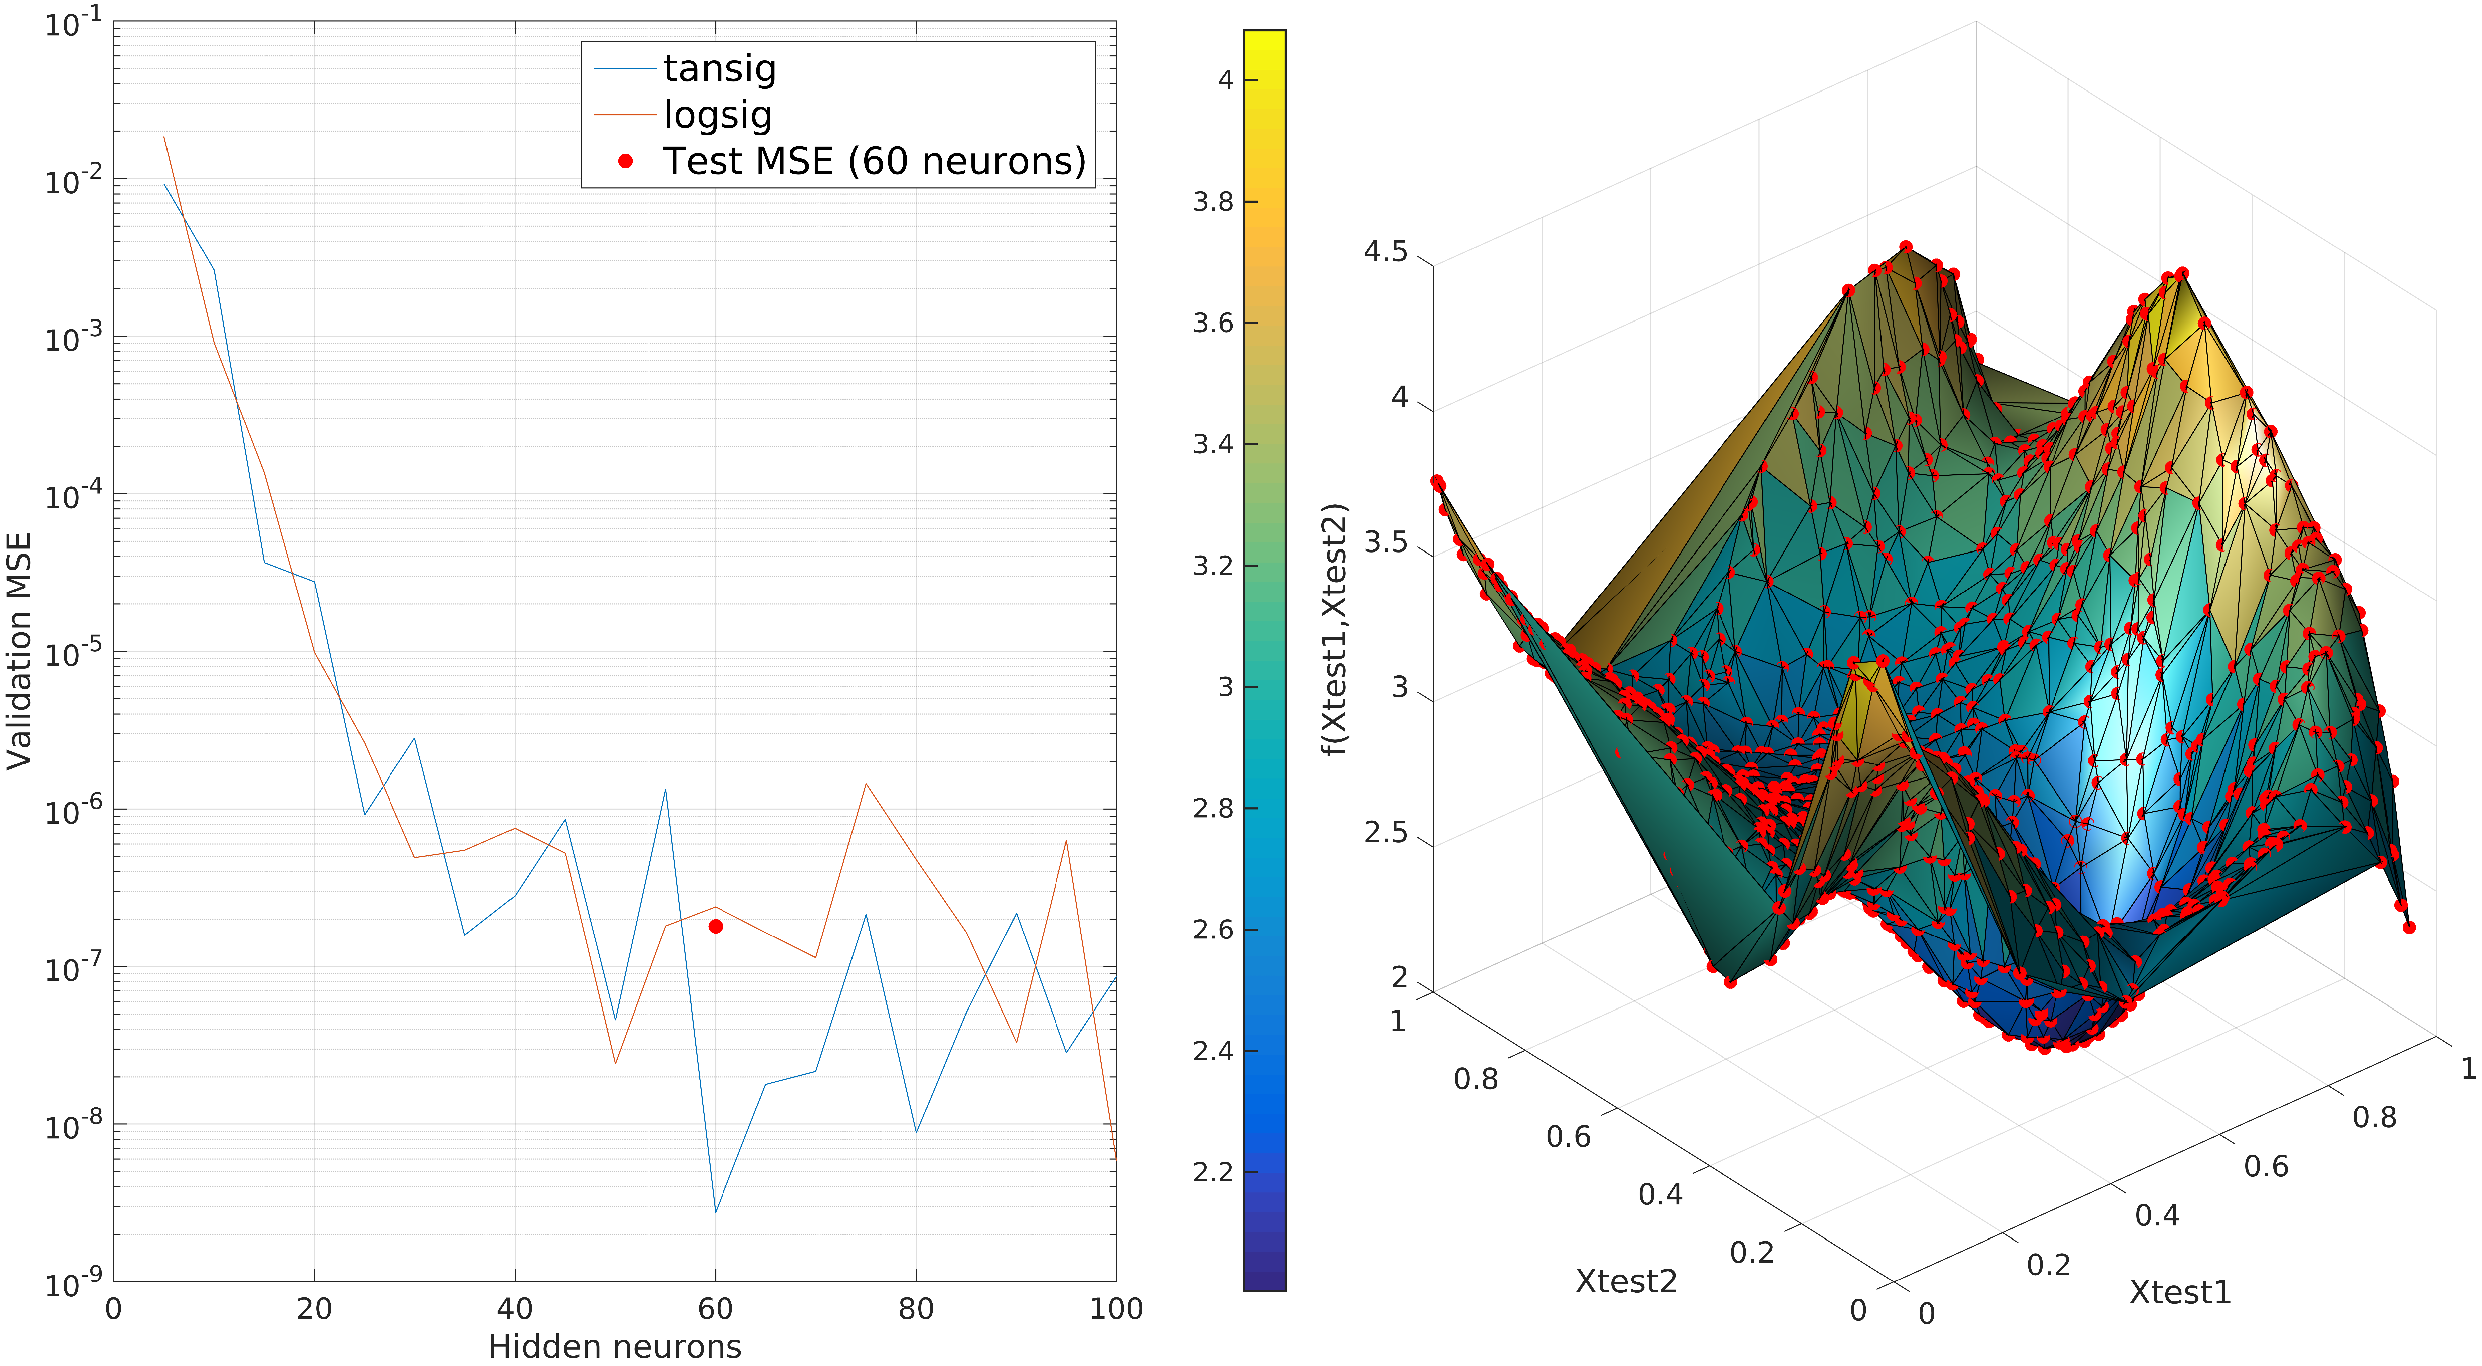
\includegraphics[scale=0.34]{regression_logtan_error.pdf}
  \caption{Validation MSE curves and test surface + prediction (red balls)}
  \label{fig:test_mse_error}
\end{figure}

Computation of the difference between the predicted values and actual
values for the test set revealed the extreme precision of the function
estimation. The errors are in the order of $10^-5$ to $10^-9$, the
largest error (in absolute value) is 0.015. Although this is indeed
excellent, it is possible to improve the process by using more of the
available data. Using cross validation on 80\% of the dataset for
example and set aside 20\% of the dataset for test purposes. 

\section{Classification}

In this section, we focus on a classification task related to red and
white wine quality. The dataset was subset according to the
instructions with my student number r0575791. Hence I had the task of
classifying white wines with positive class 6, and negative class 7.

I tried to use the \emph{feedforwardnet} but kept getting into
troubles where all the predictions of my trained network were of one
class, so I found a more modern alternative \emph{patternnet}. I first
reformulated my target, 6 and 7, as 1 and 0. This is compatible with
the sigmoid function used in the output neuron. To use this as a
classifier, one can simply take the rounded value of the output. Since
the output is always in $[0,1]$, the rounded value will be in $\{0,1\}$,
which maps naturally to the dataset.

For architecture of the network, I could not really see a large
influence in the number of hidden units (see table \ref{tab:ccr}),
there was some support for an architecture with 15 hidden units. The
training function used was the scaled conjugate gradient, default in
\emph{patternnet} since \emph{trainlm} was causing errors during the
training.

\begin{table}[H]
  \vspace{20pt}
  \centering
  \begin{tabular}{l|l|l|l|l|l|l|l|l|l|l|}
    \cline{2-11}
    & \multicolumn{1}{c|}{1} & \multicolumn{1}{c|}{2} & \multicolumn{1}{c|}{3} & \multicolumn{1}{c|}{4} & \multicolumn{1}{c|}{5} & \multicolumn{1}{c|}{10} & \multicolumn{1}{c|}{15} & \multicolumn{1}{c|}{20} & \multicolumn{1}{c|}{25} & \multicolumn{1}{c|}{30} \\ \hline
    \multicolumn{1}{|l|}{CCR\_test} & 71.75                  & 74.67                  & 72.40                  & 74.67                  & 73.37                  & 71.1                    & 75.97                   & 74.35                   & 73.05                   & 73.37                   \\ \hline
    \multicolumn{1}{|l|}{CCR\_val}  & 73.37                  & 75.00                  & 75.00                  & 75.32                  & 75.32                  & 75.32                   & 76.99                   & 76.62                   & 76.62                   & 74.67                   \\ \hline
  \end{tabular}
  \caption{Correct classification ration (test and validation) for different architectures}
  \label{tab:ccr}
\end{table}

The results of the PCA analysis are shown on figure
\ref{fig:classification_pca}. Using the rotate 3D functions in Matlab,
I could not see any evidence of obvious patterns. The first PC
explains about 30\% of the variability in the data, then it drops down
almost linearly for the next components. I selected the 6 first PC, to
have 80\%+ of the variability explained to reduce the dimension of the
dataset.

Finally, I reconstructed the dataset using these 6 components. Using
that reduced dataset, I trained another patternnet with different
numbers of hidden units. The results were less variable than in the
case above, but also a bit worse. The best CCR on the validation set
was 73.37, while the best CCR on the test set was 71.75. It would then
seem that the reduction does not impact too much the results of the
classifier, so the user/designer of the neural network in this case
could opt for it.

\begin{figure}[H]
  \centering
  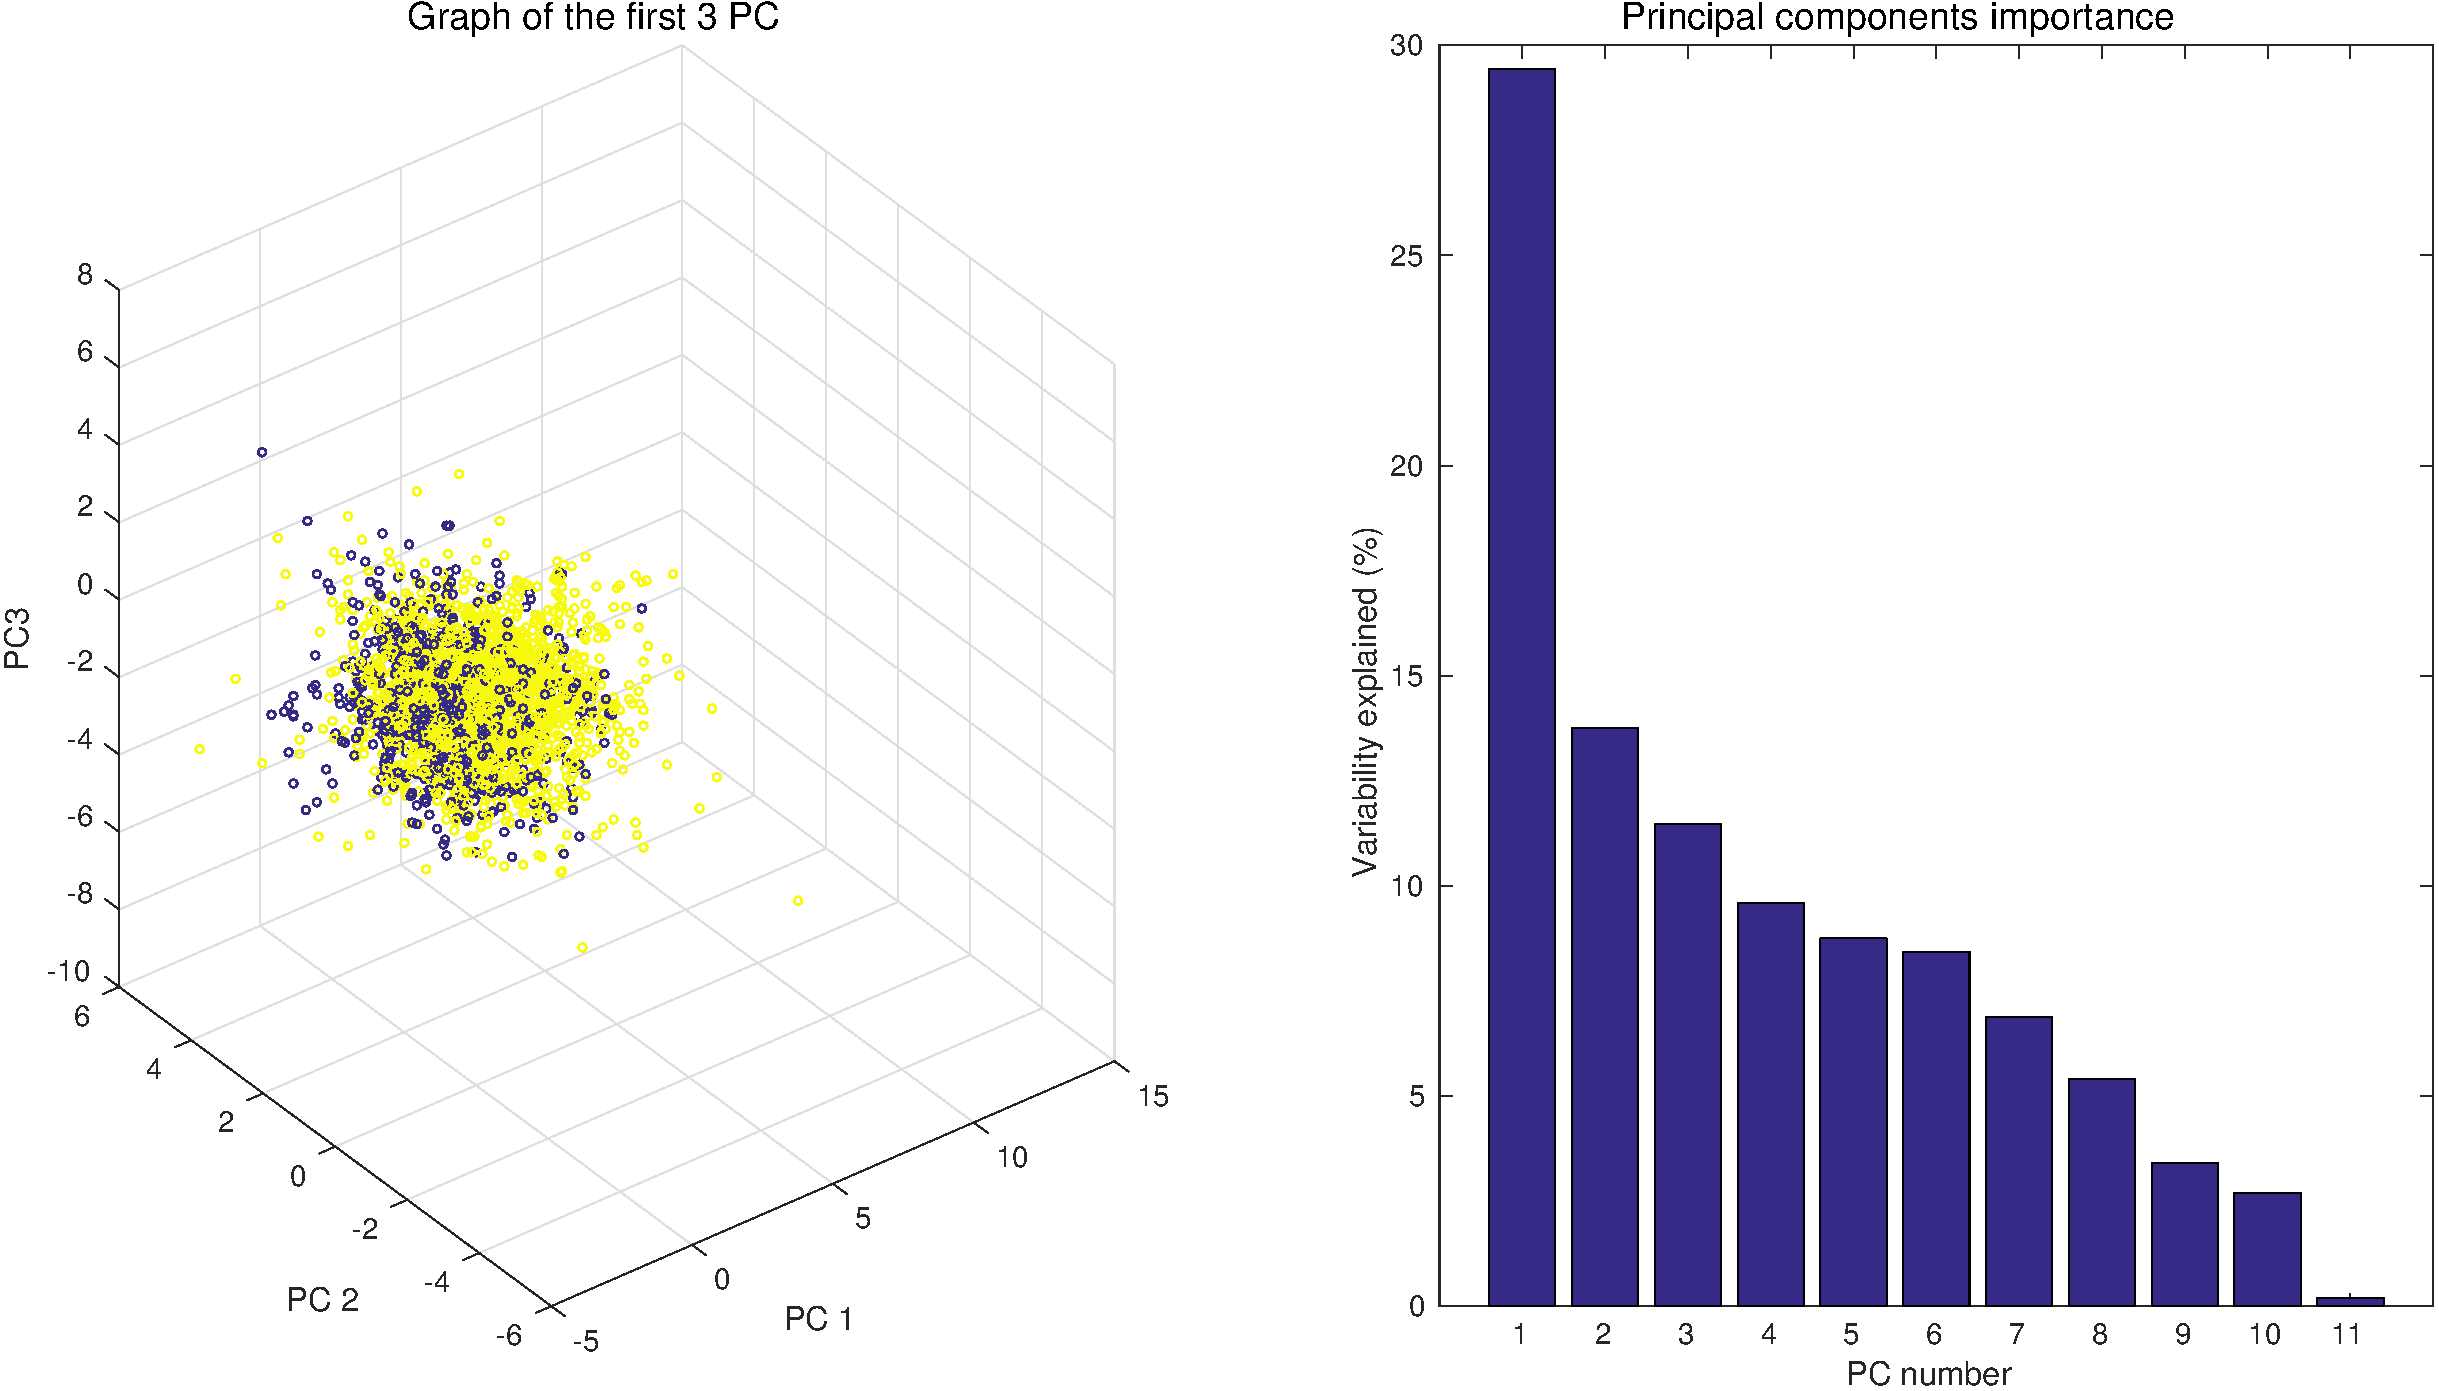
\includegraphics[scale=.35]{classification_pca.pdf}
  \caption{On the left, projection using the 3 first PC, on the right,
    the components' importance}
  \label{fig:classification_pca}
\end{figure}

\begin{appendices}
\section{Regression}
\begin{lstlisting}
clc, clear all, close all;
addpath 'export_fig'; % export pdf: https://github.com/altmany/export_fig
load '../datasets/regression.mat';

% generation of own data from student number r0575791
%%%%%%%%%%%%%%%%%%%%%%%%%%%%%%%%%%%%%%%%%%%%%%%%%%%%%
Tnew = (9*T1 + 7*T2 + 7*T3 + 5*T4 + 5*T5)/(9 + 7 + 7 + 5 + 5);

% plotting the dataset
%%%%%%%%%%%%%%%%%%%%%%
figure('Color', [1 1 1]);
tri = delaunay(X1, X2);
h = trisurf(tri, X1, X2, Tnew);
l = light('Position', [-50 -15 29]);
lighting phong; shading interp; 
colormap Jet; colorbar EastOutside;
xlabel('X1','FontSize',14); 
ylabel('X2','FontSize',14);
zlabel('f(X1,X2)','FontSize',14);

export_fig('regression_dataset.pdf');

% random permutation of the data
%%%%%%%%%%%%%%%%%%%%%%%%%%%%%%%%

dataset = [X1 X2 Tnew];
dataset = dataset(randperm(size(dataset,1)),:);
ratio = 1/3;
[trainInd, valInd, testInd] = dividerand(3000, ratio, ratio, ratio);

% training set definition
Xtrain = [dataset(trainInd,1)'; dataset(trainInd,2)'];
Ytrain = dataset(trainInd,3)';

% validation set definition
Xval = [dataset(valInd,1)'; dataset(valInd,2)'];
Yval = dataset(valInd,3)';

% test set definition
Xtest = [dataset(testInd,1)'; dataset(testInd,2)'];
Ytest = dataset(testInd,3)';

% plotting surfaces
figure('Color', [1 1 1]);

% plot train set
subplot(1,3,1);
tri = delaunay(Xtrain(:,1), Xtrain(:,2));
h = trisurf(tri, Xtrain(:,1), Xtrain(:,2), Ytrain);
l = light('Position', [-50 -15 29]);
lighting phong; colormap Jet;
xlabel('Xtrain1','FontSize',14); 
ylabel('Xtrain2','FontSize',14);
zlabel('f(Xtrain1,Xtrain2)','FontSize',14);

% plot validation set
subplot(1,3,2);
tri = delaunay(Xval(:,1), Xval(:,2));
h = trisurf(tri, Xval(:,1), Xval(:,2), Yval);
l = light('Position', [-50 -15 29]);
lighting phong; colormap Jet;
xlabel('Xval1','FontSize',14); 
ylabel('Xval2','FontSize',14);
zlabel('f(Xval1,Xval2)','FontSize',14);

% plot test set
subplot(1,3,3);
tri = delaunay(Xtest(:,1), Xtest(:,2));
h = trisurf(tri, Xtest(:,1), Xtest(:,2), Ytest);
l = light('Position', [-50 -15 29]);
lighting phong; colormap Jet; colorbar EastOutside;
xlabel('Xtest1','FontSize',14); 
ylabel('Xtest2','FontSize',14);
zlabel('f(Xtest1,Xtest2)','FontSize',14);

export_fig('regression_trainingsets.pdf');

% Estimation of number of hidden neurons
%%%%%%%%%%%%%%%%%%%%%%%%%%%%%%%%%%%%%%%%

% with sigmoid transfer function
n_hiddenn = 2:2:200;
mse_validation_logsig = zeros(100,1);
i = 1;
for nn = n_hiddenn
    net = feedforwardnet(nn);
    net.trainParam.showWindow = false;
    net.trainParam.epochs = 5000;
    net.divideFcn = 'dividetrain';
    net.layers{1}.transferFcn = 'logsig';
    net = train(net, Xtrain, Ytrain, 'UseParallel', 'yes');
    pred = sim(net, Xval);
    mse_validation_logsig(i) = perform(net, Yval, pred);
    i = i + 1;
end

% with hyperbolic tangent transfer function
n_hiddenn = 2:2:200;
mse_validation_tansig = zeros(100,1);
i = 1;
for nn = n_hiddenn
    net = feedforwardnet(nn);
    net.trainParam.showWindow = false;
    net.trainParam.epochs = 5000;
    net.divideFcn = 'dividetrain';
    net.layers{1}.transferFcn = 'tansig';
    net = train(net, Xtrain, Ytrain, 'UseParallel', 'yes');
    pred = sim(net, Xval);
    mse_validation_tansig(i) = perform(net, Yval, pred);
    i = i + 1;
end

figure('Color', [1 1 1]);
subplot(1,2,1);
semilogy(5:5:100, mse_validation_tansig);
hold on;
semilogy(5:5:100, mse_validation_logsig);
grid on;
xlabel('Hidden neurons','FontSize',14); 
ylabel('Validation MSE','FontSize',14);

% Evaluation on test set
%%%%%%%%%%%%%%%%%%%%%%%%

net = feedforwardnet(60);
net.trainParam.showWindow = true;
net.trainParam.epochs = 5000;
net.divideFcn = 'dividetrain';
net.layers{1}.transferFcn = 'tansig';
net = train(net, Xtrain, Ytrain, 'UseParallel', 'yes');
pred = sim(net, Xtest);
performance = perform(net, Ytest, pred);

hold on;
plot(60, performance, 'r*');
legend('tansig', 'logsig', 'Test MSE (60 neurons)');

export_fig('regression_logtan_error.pdf');

% Plot param selection + Plot surface of test set + prediction
%%%%%%%%%%%%%%%%%%%%%%%%%%%%%%%%%%%%%%%%%%%%%%%%%%%%%%%%%%%%%%
% tets MSE for parameter selection
figure('Color', [1 1 1]);
subplot(1,2,1);
semilogy(5:5:100, mse_validation_tansig);
hold on;
semilogy(5:5:100, mse_validation_logsig);
grid on;
xlabel('Hidden neurons','FontSize',14); 
ylabel('Validation MSE','FontSize',14);
hold on;
plot(60, performance, 'r*');
legend('tansig', 'logsig', 'Test MSE (60 neurons)');

% surface plot + prediction
subplot(1,2,2);
tri = delaunay(Xtest(1,:), Xtest(2,:));
h = trisurf(tri, Xtest(1,:), Xtest(2,:), Ytest);
l = light('Position', [-50 -15 29]);
lighting phong; colormap winter; colorbar EastOutside;
xlabel('Xtest1','FontSize',14); 
ylabel('Xtest2','FontSize',14);
zlabel('f(Xtest1,Xtest2)','FontSize',14);
hold on;
scatter3(Xtest(1,:), Xtest(2,:), pred, 'r', 'filled');
\end{lstlisting}

\section{Classification}
\begin{lstlisting}
clc, clear all, close all;
addpath 'export_fig'; % export pdf: https://github.com/altmany/export_fig
rng(7); % setting random seed

% student number = r0575791, datasets initialization
%%%%%%%%%%%%%%%%%%%%%%%%%%%%%%%%%%%%%%%%%%%%%%%%%%%%
csv_import = importdata('../datasets/winequality-white.csv');
data = csv_import.data;
cpos = data(data(:,12) == 6,:); cpos_size = length(cpos);
cneg = data(data(:,12) == 7,:); cneg_size = length(cneg);

X = [cpos(:,1:(end-1)) ; cneg(:,1:(end-1))]'; % label removed (6,7)
Y = [ones(cpos_size,1) ; zeros(cneg_size, 1)]'; % replaced by 1 and 0
stdx = mapstd(X);

% creation of training, validation, and test sets
n = cpos_size + cneg_size; 
[train_ind, val_ind, test_ind] = dividerand(n, 0.8, 0.1, 0.1);

% Neural net training
%%%%%%%%%%%%%%%%%%%%%
i = 1; ccr_val = zeros(10,1); ccr_test = zeros(10,1);
for hnn = [1 2 3 4 5 10 15 20 25 30]
    net = patternnet(hnn);%
    net.divideFcn = 'divideind';
    net.trainParam.showWindow = false;
    net.divideParam.trainInd = train_ind;
    net.divideParam.valInd = val_ind;
    net.divideParam.testInd = test_ind;
    net = train(net, stdx, Y);

    pred = round(sim(net, stdx(:,val_ind)));
    ccr_val(i) = sum(pred == Y(:,val_ind))*100/length(val_ind);
    pred = round(sim(net, stdx(:,test_ind)));
    ccr_test(i) = sum(pred == Y(:,test_ind))*100/length(test_ind);
    i = i + 1;
end

% PCA
%%%%%
[coeff,scores,~,~,explained] = pca(X(:,train_ind)','Centered', true, 'VariableWeights','variance');
figure('Color',[1 1 1]);
subplot(1,2,1);
scatter3(scores(:,1), scores(:,2), scores(:,3), 15, Y(train_ind));
title('Graph of the first 3 PC'); xlabel('PC 1'); ylabel('PC 2'); zlabel('PC3');
subplot(1,2,2);
bar(explained);
title('Principal components importance'); xlabel('PC number'); ylabel('Variability explained (%)');

% reconstruction of whole dataset with 6 components
reduced_dim = coeff(:,1:6);
reduced_data = X' * reduced_dim;
reduced_data = reduced_data';
stdxr = reduced_data;%mapstd(reduced_data);

i = 1; ccr_val = zeros(10,1); ccr_test = zeros(10,1);
for hnn = [1 2 3 4 5 10 15 20 25 30]
    net = patternnet(hnn);%
    net.divideFcn = 'divideind';
    net.trainParam.max_fail = 50;
    net.trainParam.min_grad=1e-10;
    net.trainParam.showWindow = true;
    net.divideParam.trainInd = train_ind;
    net.divideParam.valInd = val_ind;
    net.divideParam.testInd = test_ind;
    net = train(net, stdxr, Y);

    pred = round(sim(net, stdxr(:,val_ind)));
    ccr_val(i) = sum(pred == Y(:,val_ind))*100/length(val_ind);
    pred = round(sim(net, stdxr(:,test_ind)));
    ccr_test(i) = sum(pred == Y(:,test_ind))*100/length(test_ind);
    i = i + 1;
end

[max_ccr_test, pos_test] = max(ccr_test);
[max_ccr_val, pos_val] = max(ccr_val);
\end{lstlisting}
\end{appendices}
\end{document}
